\section{Basics}
\label{sec:eventdriven_basics}
In this section we derive the basics of event-driven ABS using the SIR model, as introduced in Chapter \ref{sec:sir_model}, with an event-driven approach inspired by \cite{macal_agent-based_2010}. Although it is a fundamentally different approach to ABS than the time-driven implementation in Chapter \ref{sec:timedriven_firststep}, both solutions are quantitatively equal as they produce the same class of dynamics. Qualitatively they differ in terms of expressivity and performance as we will see in the discussion.

The basics of event-driven ABS are the concept of agent identity, events and event scheduling. We introduce them step-by-step using various Monads and then generalise to a \textit{tagless final} approach, which has various benefits as pointed out in the respective section. 

\subsection{An Event-Driven SIR}
Before we can derive implementation concepts, we first need to discuss how an event-driven SIR model works, as inspired by \cite{macal_agent-based_2010}. Fundamentally, what is required is to transform all time-dependent behaviour and agent interactions into the scheduling and receiving of events. For the SIR this should be trivial and straightforward, taking inspiration from the time-driven implementation, where we simply translate the occurrences of events generated by \texttt{occasionally} into scheduling of events. For agent interactions we also use events, making this more explicit than in the time-driven approach. As already pointed out, assuming that events have a receiver and a scheduling time given as $\Delta t$ relative to the current simulation time, we end up with three event types:

\begin{enumerate}
	\item \textbf{MakeContact} is used to let susceptible agents proactively make contact with $\beta$ (contact rate) other agents per time unit.
	\item \textbf{Contact$_{Sender, \ SIRState}$} is used to make contact between agents where, agents reveal their state by sending or replying with their current state.
	\item \textbf{Recover} is used to let infected agents recover proactively after the given $\delta$ (illness duration). 
\end{enumerate}

Now we can give a concise definition of all three agent behaviours:

\paragraph{Susceptible Agent}
\begin{itemize}
	\item A susceptible agent initially schedules a \texttt{MakeContact} event with $\Delta t = 1$ to itself.
	
	\item When receiving \texttt{MakeContact}, the agent sends a \texttt{Contact} event to $\beta$ (contact rate) random other agents with $\Delta t = 0$ and the \texttt{SIRState} of \texttt{Susceptible}, resulting in these events being scheduled immediately. Furthermore, the agent schedules \texttt{MakeContact} with $\Delta t = 1$ to itself, to keep the proactive process of making contact with other agents active.
	
	\item When the agent receives a \texttt{Contact} event, it checks if this is from an infected agent (\texttt{SIRState} is \texttt{Infected}). If the event is not from an infected agent, it ignores it, otherwise it becomes infected with a given probability.
\end{itemize}

\paragraph{Infected Agent}
\begin{itemize}
	\item An infected agent initially schedules a \texttt{Recover} event to itself, with an exponentially distributed random $\Delta t$ of $\delta$ (illness duration).
	
	\item When the agent receives a \texttt{Contact} event, it checks if it is from a susceptible agent (\texttt{SIRState} is \texttt{Susceptible}). If the event is not from a susceptible agent, it ignores it, otherwise it simply replies to the same susceptible agent with a \texttt{Contact} event with $\Delta t = 0$ and and \texttt{SIRState} of \texttt{Infected}.
\end{itemize}

\paragraph{Recovered Agent}
The recovered agent does not change anymore, reacts to no incoming events and schedules no events - it stays constantly \texttt{Recovered} forever.

\medskip

It is easy to see that this behaviour emulates the time-driven one and indeed in Figure \ref{fig:sir_eventdriven_dynamics} it is also visually clear that it produces similar dynamics. A striking difference are the small spikes and steps in the dynamics. This differences stem from the fact that time advances discretely and not continuously as in the time-driven implementation. In Chapter \ref{ch:sir_invariants}, we use property-based testing to show that both implementations indeed produce similar distributions in their dynamics, thus putting the claim that both implementations are quantitatively equal on a much more robust ground.

\begin{figure}
	\centering
	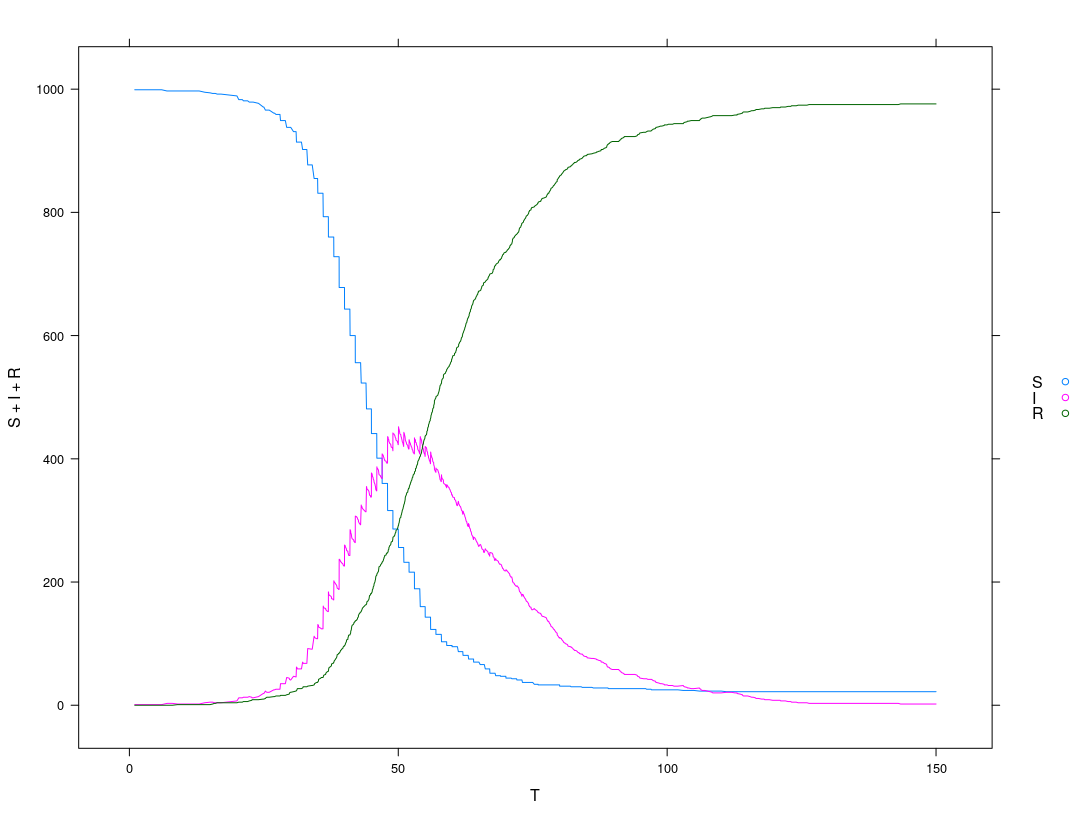
\includegraphics[width=0.7\textwidth, angle=0]{./fig/eventdriven/sir_eventdriven.png}
	\caption[Dynamics of the event-driven SIR model]{Dynamics of the event-driven SIR model. Population Size $N$ = 1,000, contact rate $\beta = \frac{1}{5}$, infection probability $\gamma = 0.05$, illness duration $\delta = 15$ with initially 1 infected agent. Simulation run for 150 time steps.}
	\label{fig:sir_eventdriven_dynamics}
\end{figure}

\subsection{Events, agent identity and scheduling}
We can now start to discuss the concepts from an implementation perspective. First, we need to make the concept of an event explicit. An event is of a given type, has a receiver and a timestamp in \textit{absolute} simulation time when it shall be scheduled. We keep the event type polymorphic and represent the receiver by an \texttt{AgentId} which is a simple \texttt{Int}. For efficient scheduling, the events are kept in a priority queue \href{http://hackage.haskell.org/package/pqueue}{Data.PQueue.Min}~\cite{pqueue_library}, sorted ascending by the timestamp. Thus, we define the following:

\begin{HaskellCode}
type Time        = Double
type AgentId     = Int
data QueueItem e = QueueItem e AgentId Time

-- the event priority queue
type EventQueue e = PQ.MinQueue (QueueItem e)

-- implement Ord for QueueItem for acended sorting
instance Ord (QueueItem e) where
  compare (QueueItem _ _ t1) (QueueItem _ _ t2) = compare t1 t2
\end{HaskellCode}

Next, we define a polymorphic type for the agent. In event-driven ABS, due to the fact that agents are not signals anymore, we abandon time-aware signal functions of BearRiver from the previous chapter and focus solely on MSF. In event-driven ABS agents receive events, thus as input to an \texttt{MSF} the polymorphic event type \texttt{e} is used. As output, the polymorphic output type \texttt{o} is used, which will be instantiated to a specific monomorphic type in the SIR model below. The question now becomes what Monad shall be used? For scheduling purposes (and because models might require it), agents should be able to \textit{read} the current simulation time: this is accomplished through a \texttt{ReaderT Time}. Furthermore, agents should be able to \textit{read} the identities of the other agents available in the simulation so they can schedule events to them when necessary, which is accomplished through a \texttt{ReaderT [AgentId]}. Most importantly, agents have to be able to schedule events. This means they have to be able to \textit{write} the events into some sink where they are accumulated for scheduling, which is achieved through a \texttt{WriterT [QueueItem e]}. Finally, the transformer stack needs to be extendible by other Monads, specified in concrete models like the SIR below. As such we add another polymorphic type \texttt{m}, indicating the closing Monad (stack).

\begin{HaskellCode}
type ABSMonad m e   = ReaderT Time (WriterT [QueueItem e] (ReaderT [AgentId] m))
type AgentMSF m e o = MSF (ABSMonad m e) e o
\end{HaskellCode}

BearRivers \texttt{SF} also has a \texttt{ReaderT Double} as the outermost Monad but we deliberately avoided its use because the intended semantics of an \texttt{SF} are different. The value in the \texttt{ReaderT} of the \texttt{SF} represents the sampling time delta and not the absolute time, as in the event-driven case.

We can already implement a few polymorphic functions, operating on the given Monad stack. First, we implement the function \texttt{allAgentIds} which simply returns the \texttt{AgentId} of all agents, for the scheduling of a given event to a given receiver into the future given a specific time delay, relative to the current simulation time.
 
\begin{HaskellCode}
allAgentIds :: Monad m => (ABSMonad m e) [AgentId]
allAgentIds = lift (lift ask)

scheduleEvent :: Monad m
              => e        -- event
              -> AgentId  -- receiver
              -> Double   -- time delay
              -> (ABSMonad m e) ()
scheduleEvent e aid dt = do
  -- get current simulation time
  t <- ask
  -- construct queue item
  let q = QueueItem e aid (t + dt)
  -- write/append (tell) to the WriterT (QueueItem e)
  lift (tell [q])
\end{HaskellCode}

Processing events can also be implemented generically and is straightforward. Therefore, we only discuss it conceptually. For efficient lookup of event receivers all agents are organised into an \texttt{IntMap}, which also holds the current output of the agent, to allow sampling of the domain state. In general, the domain state is highly model specific, thus a generic implementation needs to offer some mechanism to update the domain state after an event. We named this process \textit{domain state sampling}. Our approach is to call a function which receives the agent map and returns a new domain state for the current event or time step. These domain states are appended to an infinite list which forms the output of the simulation.

The events are then processed in the order provided by the queue and each event is executed with the given receiver. Running a receiver is simply achieved using the agent map, where a reviver is looked up and its \texttt{MSF} is evaluated with the given event as input and the resulting monadic actions executed with the given parameters.
 
\subsection{Parametrising for SIR}
With the generic concepts now established, we show how to parametrise them to the concrete SIR model. First, we define the already well-known states the agents can be in and the three different event types, as already introduced above.

\begin{HaskellCode}
data SIRState = Susceptible | Infected | Recovered
data SIREvent = MakeContact | Contact AgentId SIRState | Recover 
\end{HaskellCode}

Next, we parametrise the \texttt{ABSMonad} to the SIR model. Because behaviour is stochastic, we need to make use of the \texttt{Rand} Monad, which also closes the Monad stack of \texttt{ABSMonad}. Further, the event type is obviously parametrised to \texttt{SIREvent}.

\begin{HaskellCode}
type SIRMonad g = ABSMonad (Rand g) SIREvent
\end{HaskellCode}

Now we define a \texttt{SIRAgent} which can be understood as a constructing function, run once upon construction of the agent. This constructing function runs in the \texttt{SIRMonad}, thus agents can already make full use of the functionality. So they can schedule initial events, depending on their initial state. This is important for the susceptible and infected agent, which both need to schedule initial events for their proactive behaviour. The constructing function also takes the \texttt{AgentId} of the agent, thus making it available to the agent at construction time. It returns the initial agent behaviour as \texttt{AgentMSF}.

\begin{HaskellCode}
type SIRAgent g 
       = AgentId -> (SIRMonad g) (AgentMSF (SIRMonad g) SIREvent SIRState)
\end{HaskellCode}

The implementation of the constructing function of type \texttt{SIRAgent} is straightforward and follows the specification given above. It makes use of the functions \texttt{scheduleMakeContact} and \texttt{scheduleRecovery} which are implemented using the generic \texttt{scheduleEvent} from above.

\begin{HaskellCode}
sirAgent :: RandomGen g 
         => Int         -- ^ contact rate (beta)
         -> Double      -- ^ infectivity (gamma)
         -> Double      -- ^ illness duration (delta)
         -> SIRState    -- ^ initial state of the agent
         -> SIRAgent g
sirAgent beta gamma delta Susceptible aid = do
  -- on start, schedule MakeContact to itself
  scheduleMakeContact aid 1
  -- return susceptible behaviour
  return (susceptibleAgent aid beta gamma delta)
sirAgent _ _ delta Infected aid = do
  -- on start, schedule Recover to itself
  scheduleRecovery aid delta
  -- return infected behaviour
  return (infectedAgent aid)
sirAgent _ _ _ Recovered _ = 
  -- simply return recovered behaviour
  return recoveredAgent

scheduleMakeContact :: RandomGen g => AgentId -> Double -> (SIRMonad g) ()
scheduleMakeContact aid = scheduleEvent MakeContact aid

scheduleRecovery :: RandomGen g => AgentId -> Double -> (SIRMonad g) ()
scheduleRecovery aid delta = do
  dt <- (lift . lift . lift) (randomExpM (1 / delta))
  scheduleEvent Recover aid dt

-- returns random value following exponential distribution with given lambda
randomExpM :: MonadRandom m => Double -> m Double
\end{HaskellCode}

Now we are finally ready to implement the actual behaviour of an agent, where we discuss the full implementation of the susceptible agent behaviour. The basic structure should be already familiar from the time-driven approach, using \texttt{switch} to dynamically change the behaviour to \texttt{infectedAgent} in case of an infection. The behaviour is then a simple event handler, pattern matching on the incoming events:

\begin{HaskellCode}
susceptibleAgent :: RandomGen g 
                 => AgentId        -- agents id
                 -> Int            -- contact rate (beta)
                 -> Double         -- infectivity (gamma)
                 -> Double         -- illness duration (delta)
                 -> SIRAgentMSF g
susceptibleAgent aid beta gamma delta = 
    switch susceptibleAgentInfected (const (infectedAgent aid))
  where
    susceptibleAgentInfected :: RandomGen g 
                             => MSF (SIRMonad g) SIREvent (SIRState, Maybe ()) 
    susceptibleAgentInfected = proc e -> do
      -- handle incoming event in monadic action
      ret <- arrM handleEvent -< e
      case ret of
        Nothing -> returnA -< (Susceptible, ret)
        _       -> returnA -< (Infected, ret)
\end{HaskellCode}

We strictly follow the specification as above. In case the agent receives \texttt{Contact} from an infected agent it might become infected with a given probability. If it becomes infected, it schedules the recovery as it will make the transition to an infected agent.

\begin{HaskellCode}
handleEvent :: RandomGen g => SIREvent -> (SIRMonad g) (Maybe ())
handleEvent (Contact _ Infected) = do
  -- become infected with gamma probability
  r <- (lift . lift . lift) (randomBoolM gamma)
  if r
    -- got infected 
    then do
      -- schedule Recovery to self, because switching to infected
      scheduleRecovery aid delta
      return (Just ())
    -- no infection
    else return Nothing

-- returns True with given probability
randomBoolM :: MonadRandom m => Double -> m Bool
\end{HaskellCode}

In case the agent receivers \texttt{MakeContact} from itself, it will send \texttt{Contact} with \texttt{Susceptible} to $\beta$ (contact rate) other agents without delay and \texttt{MakeContact} to itself with a delay of 1 time unit.

\begin{HaskellCode}
handleEvent MakeContact = do
  ais <- allAgentIds
  -- get beta random agents
  receivers <- (lift . lift . lift) (forM [1..beta] (const (randomElemM ais)))
  -- make contact with random agents
  mapM_ makeContactWith receivers
  -- reschedule MakeContact to self
  scheduleMakeContact aid 1
  return Nothing
  
makeContactWith :: AgentId -> (SIRMonad g) ()
makeContactWith receiver = 
  -- schedule Contact event immediately
  scheduleEvent (Contact aid Susceptible) receiver 0

-- picks an element randomly from the (non empty) list
randomElemM :: MonadRandom m => [e] -> m e
\end{HaskellCode}

The infected and recovered behaviours are conceptually equivalent and thus left as a trivial exercise to the reader. 

\subsection{Tagless Final}
\label{sec:tagless_final_basics}
At this point, the basics of event-driven ABS have been established: how events are represented and processed using an event queue, how agents are represented with an \texttt{MSF} and the idea behind the underlying polymorphic Monad Transformer stack. Furthermore, by parametrising the polymorphic concepts to the SIR model, we showed how to instantiate the generic concepts into a concrete model. Thus, we arrived at a robust, maintainable, and solid solution which is very likely to be correct up to the initial informal specification.

\medskip

In this section we briefly want to show how the so-called \textit{tagless final} approach \cite{kiselyov_typed_2012} can be used to arrive at a cleaner and more extensible \textit{interface} of our implementation, which is also open to different \textit{interpretations}. The idea behind tagless final is simple: specify the interface of operations in a type class and then write one or multiple interpreters for it, which simply means writing an instance implementation for the given type class. We start by defining the type class \texttt{MonadAgent} with all the necessary methods, making up the effectful API of our agents. We need to enable two language extensions: \texttt{MultiParamTypeClasses} because we want to have more than a single type parameter in the type class: besides the Monad \texttt{m}, we also want to parametrise over the event type \texttt{e}; \texttt{FunctionalDependencies} because the event type \texttt{e} is determined by the Monad type \texttt{m}.

\begin{HaskellCode}
class Monad m => MonadAgent e m | m -> e where
  randomBool  :: Double -> m Bool
  randomExp   :: Double -> m Double
  randomElem  :: [a] -> m a
  getAgentIds :: m [AgentId]
  getTime     :: m Time
  getMyId     :: m AgentId
  schedEvent  :: e -> AgentId -> Double -> m ()
\end{HaskellCode}

This type class is now used to replace the Monad stack by an overloaded type definition in the respective functions. Thus, the implementation of the agent constructing function and the agent behaviours are the same, with only the types changing slightly, lifts becoming obsolete and calls to function replaced by calls to methods of the type class. We don't give the full implementation again but only the type of the agent construction function as example, the types of the agent behaviours follow a similar pattern: 

\begin{HaskellCode}
sirAgent :: MonadAgent SIREvent m       -- CHANGED: overloaded with type class
         => Int                         -- contact rate (beta)
         -> Double                      -- infectivity (gamma)
         -> Double                      -- illness duration (delta)
         -> SIRState                    -- initial state of the agent
         -> m (MSF m SIREvent SIRState) -- CHANGED: no Monad stack
\end{HaskellCode}

We added a \texttt{getMyId} method, which returns the \texttt{AgentId} of the agent itself, avoiding the need for the agent of keeping the agent id around and also making it possible to implement more robust self-scheduling functions. For example, the \texttt{scheduleRecovery} function is implemented in the tagless final approach in the following way:

\begin{HaskellCode}
scheduleRecovery :: MonadAgent SIREvent m => Double -> m ()
scheduleRecovery delta = do
  -- draw random value from exponential distribution
  dt <- randomExp (1 / delta)
  -- get id of agent, no more need to pass it explicitly
  ai <- getMyId
  -- schedule Recover to itself
  schedEvent Recover ai dt
\end{HaskellCode}

What we are missing is a \textit{pure} interpreter for the agent implementation and the \texttt{MonadAgent} type class. We start by defining a \texttt{newtype}, which basically is a conceptually similar Monad stack as in the original implementation without the tagless final approach. We let Haskell automatically derive monadic type classes, Functor, Applicative and Monad instances which saves a lot of boiler plate code, for which the \texttt{GeneralizedNewtypeDeriving} language extension is required. Instead of the \texttt{Rand} Monad, a \texttt{StateT SimState} is used, which carries the random number generator and other data for synchronous agent interactions as will be discussed in the sections on advanced features.

\begin{HaskellCode}
newtype SIRAgentPure a = SIRAgentPure 
  { unSirAgentPure :: ReaderT (Time, AgentId, [AgentId]) -- combined into one
                        (WriterT [QueueItem SIREvent]
                          (State SimState)) a}
  deriving (Functor, Applicative, Monad, 
            MonadReader (Time, AgentId, [AgentId]),
            MonadWriter [QueueItem SIREvent],  
            MonadState SimState)
\end{HaskellCode}

Having this \texttt{newtype} we can now write a \textit{pure} interpreter for the \texttt{MonadAgent}. The implementations is straightforward and should be self-explanatory. To run the existing \texttt{Rand} Monad actions, the function \texttt{runRandWithSimState} is used, which extracts the random-number generator from \texttt{SimState}, runs the action and puts the changed random-number generator back into the \texttt{SimState}.

\begin{HaskellCode}   
instance MonadAgent SIREvent SIRAgentPure where
  randomBool = runRandWithSimState . randomBoolM
  randomElem = runRandWithSimState . randomElemM
  randomExp  = runRandWithSimState . randomExpM
  -- schedEvent :: SIREvent -> AgentId -> Double -> m ()
  schedEvent e receiver dt = do
    t <- getTime 
    tell [QueueItem e receiver (t + dt)]
  -- getAgentIds :: m [AgentId]
  getAgentIds = asks trd
  -- getTime :: m Time
  getTime = asks fst3
  -- getMyId :: m AgentId
  getMyId = asks snd3

fst3 :: (a,b,c) -> a
snd3 :: (a,b,c) -> b
trd :: (a,b,c) -> c
runRandWithSimState :: MonadState SimState m => Rand StdGen a -> m a
\end{HaskellCode}

The main benefit of a tagless final approach is that it is a solution to the expression problem \cite{kiselyov_typed_2012}, which allows us to add new interpreters of an embedded language and add new functionality without breaking the existing implementations. Interpretation in our case means that we can use different underlying Monads to run the agents. When we want to guarantee purity, no \texttt{IO} Monad must be used. Otherwise, when concurrency with a lock-based or lock-free approach is required \texttt{IO} or \texttt{STM} can be used in the underlying interpreter. Additionally, for reproducible unit testing, one can write custom test interpreters where methods always return a-priori known results, similar to mocking. Adding new functionality is discussed in the next section and also might become highly important when designing a more general ABS library, building on the tagless final approach. It would allow the user of such a library to extend existing agents or default behaviour with new, custom-built methods, without breaking the existing ones. We leave that for further research.